%% start of file `template.tex'.
%% Copyright 2006-2013 Xavier Danaux (xdanaux@gmail.com).
%
% This work may be distributed and/or modified under the
% conditions of the LaTeX Project Public License version 1.3c,
% available at http://www.latex-project.org/lppl/.


\documentclass[11pt,a4paper,sans]{moderncv}        % possible options include font size ('10pt', '11pt' and '12pt'), paper size ('a4paper', 'letterpaper', 'a5paper', 'legalpaper', 'executivepaper' and 'landscape') and font family ('sans' and 'roman')

% moderncv themes
\moderncvstyle{banking}                            % style options are 'casual' (default), 'classic', 'oldstyle' and 'banking'
\moderncvcolor{red}                                % color options 'blue' (default), 'orange', 'green', 'red', 'purple', 'grey' and 'black'
%\renewcommand{\familydefault}{\sfdefault}         % to set the default font; use '\sfdefault' for the default sans serif font, '\rmdefault' for the default roman one, or any tex font name
%\nopagenumbers{}                                  % uncomment to suppress automatic page numbering for CVs longer than one page

% character encoding
\usepackage[utf8]{inputenc}                       % if you are not using xelatex ou lualatex, replace by the encoding you are using
%\usepackage{CJKutf8}                              % if you need to use CJK to typeset your resume in Chinese, Japanese or Korean

% adjust the page margins
\usepackage[scale=0.75]{geometry}
%\setlength{\hintscolumnwidth}{3cm}                % if you want to change the width of the column with the dates
%\setlength{\makecvtitlenamewidth}{10cm}           % for the 'classic' style, if you want to force the width allocated to your name and avoid line breaks. be careful though, the length is normally calculated to avoid any overlap with your personal info; use this at your own typographical risks...


% personal data
\name{David}{Ayodele}
\title{Cover Letter}                               % optional, remove / comment the line if not wanted
\address{948 West Libra Drive}{Tempe, AZ 85283}{USA}% optional, remove / comment the line if not wanted; the "postcode city" and and "country" arguments can be omitted or provided empty
% \phone[mobile]{+1~(234)~567~890}                   % optional, remove / comment the line if not wanted
\phone[fixed]{+1~(602)~824~8091}                    % optional, remove / comment the line if not wanted
% \phone[fax]{+3~(456)~789~012}                      % optional, remove / comment the line if not wanted
\email{dav2092098@maricopa.edu}                               % optional, remove / comment the line if not wanted
% \homepage{www.johndoe.com}                         % optional, remove / comment the line if not wanted
% \extrainfo{additional information}                 % optional, remove / comment the line if not wanted
\photo[64pt][0.4pt]{picture}                       % optional, remove / comment the line if not wanted; '64pt' is the height the picture must be resized to, 0.4pt is the thickness of the frame around it (put it to 0pt for no frame) and 'picture' is the name of the picture file
\quote{Some quote}                                 % optional, remove / comment the line if not wanted

% to show numerical labels in the bibliography (default is to show no labels); only useful if you make citations in your resume
%\makeatletter
%\renewcommand*{\bibliographyitemlabel}{\@biblabel{\arabic{enumiv}}}
%\makeatother
%\renewcommand*{\bibliographyitemlabel}{[\arabic{enumiv}]}% CONSIDER REPLACING THE ABOVE BY THIS

% bibliography with mutiple entries
%\usepackage{multibib}
%\newcites{book,misc}{{Books},{Others}}
%----------------------------------------------------------------------------------
%            content
%----------------------------------------------------------------------------------
\begin{document}
%-----       letter       ---------------------------------------------------------
% recipient data
\recipient{Mike Van Gels}{Gordian Networks\\2151 E. Broadway Rd. \#115\\Tempe, AZ 85282}
\date{May 01, 2018}
\opening{Hello and thank you for time,}
\closing{}
\enclosure[Attached]{Resumé}          %  vit\ae{} use an optional argument to use a string other than "Enclosure", or redefine \enclname
\makelettertitle


Ms. Jessica Bradford recently contacted me with information about your company and the IT technician position opening. In looking further into your company and the position opening, the position appears to be within my qualifications and working with your company seems like an exciting opportunity.

Having a background in shipping and receiving, as well in logistics, database
programming, and web development, I feel I would be able to contribute to your organization.
Some relevant skills I possess are in such areas as processing orders (incoming and
outgoing orders), preparing shipments, organizing work orders, building and maintaining websites and web-based applications. I have experience using various mechanical lifts and special shipping equipment. I am experienced in working with customers to process returns, resolve complaints, and provide responses to general inquiries in a timely and courteous manner. I am additionally proficient in maintaining records with SQL, MS Excel, VBA,
and have written many scripts in VBA for customer data organization.
\newline
\newline
I am confident I can be a valuable asset to your organization and would be delighted to
interview for the position.\newline \newline \newline \\ 


Thank you,


% Albert Einstein discovered that $e=mc^2$ in 1905.
%\[ e=\lim_{n \to \infty} \left(1+\frac{1}{n}\right)^n \]
\begin{minipage}{\textwidth}
  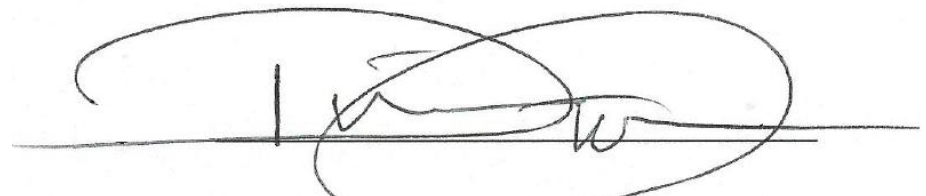
\includegraphics[width=0.5\textwidth]{sig.png} \\
\end{minipage}
\makeletterclosing

\end{document}


%% end of file `template.tex'.
